\section{Auswertung}
\label{sec:Auswertung}
\subsection{Subtraktion des Untergrundes von den Messwerten}
Zunächst werden die Messwerte für den Anlaufstrom von systematischen Untergrundströmen bereinigt. Der gemessene Untergrundstrom für die jeweiligen Messungen lautet:
\begin{center}
  $I_{0,1} = \SI{0.2}{\pico\ampere}$, $I_{0,2} = \SI{-0.15}{\pico\ampere}$.
\end{center}
Das Vorzeichen des Stromes steht hierbei für die Stromrichtung.\\
Damit möglichst genaue Ergebnisse erzielt werden, werden die aufgenommenen Werte für Strom und Temperatur von weiterem Untergrund getrennt. Durch eine exponentielle Regression der Messwerte um die Minima der in Abbildung \ref{fig:mitunter} dargestellten Daten, wird dieser Untergrund approximiert.
Anschließend wird er von allen Messwerten abgezogen, wodurch sich die Kurven aus Abbildung \ref{fig:ohneunter} ergeben.\\
\begin{figure}[H]
  \centering
  \begin{subfigure}{0.48\textwidth}
    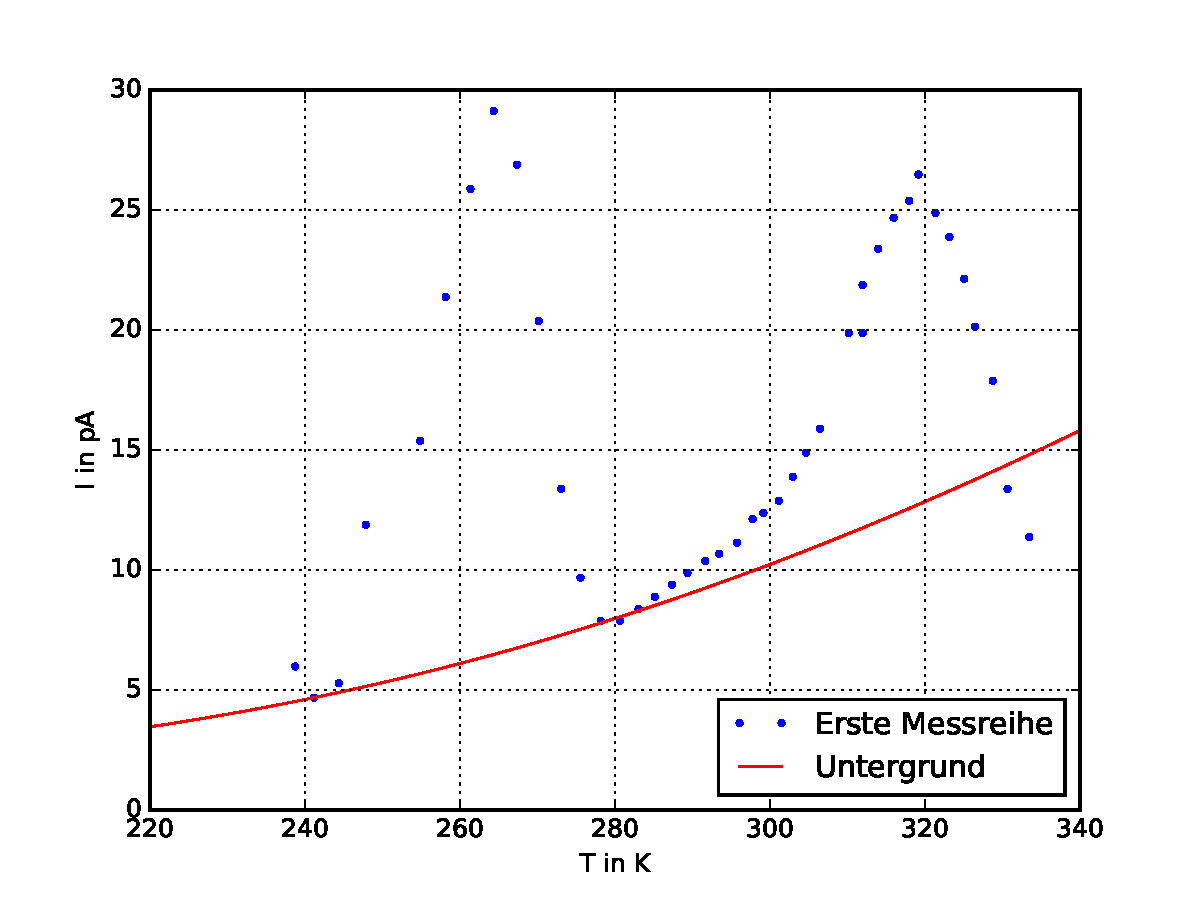
\includegraphics[height=6.2cm]{plots/mituntergrund.pdf}
    \caption{Messreihe 1}
    \label{fig:mess1}
  \end{subfigure}
  \begin{subfigure}{0.48\textwidth}
    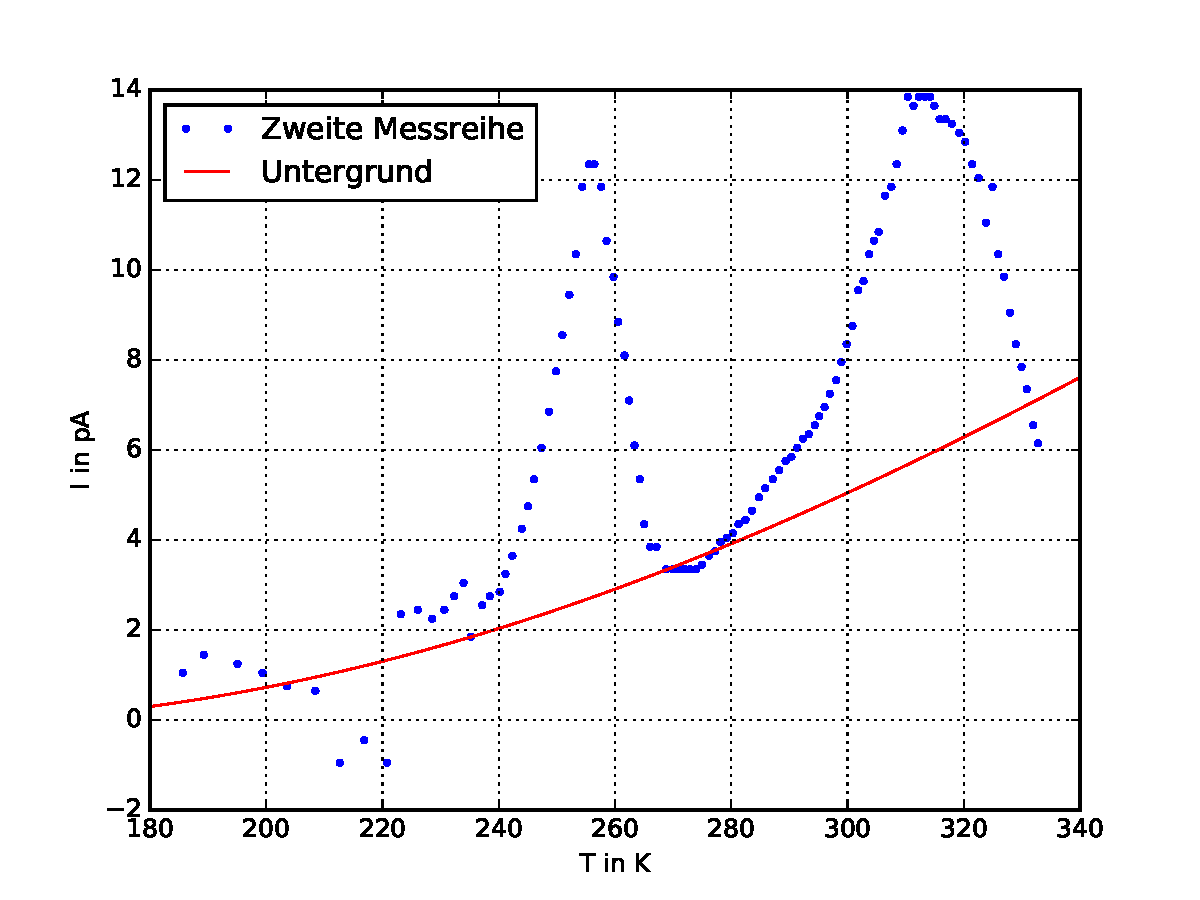
\includegraphics[height=6.2cm]{plots/mituntergrund2.pdf}
    \caption{Messreihe 2}
    \label{fig:mess2}
  \end{subfigure}
  \caption{Aufgenommene Messwerte für die 2 verschiedenen Heizraten. Es ist der  Strom in Abhängigkeit von der Temperatur aufgetragen. Zusehen ist außerdem die Ausgleichsrechnung  für den abzuziehenden Untergrund.}
  \label{fig:mitunter}
\end{figure}
\begin{figure}[H]
  \begin{subfigure}{0.48\textwidth}
   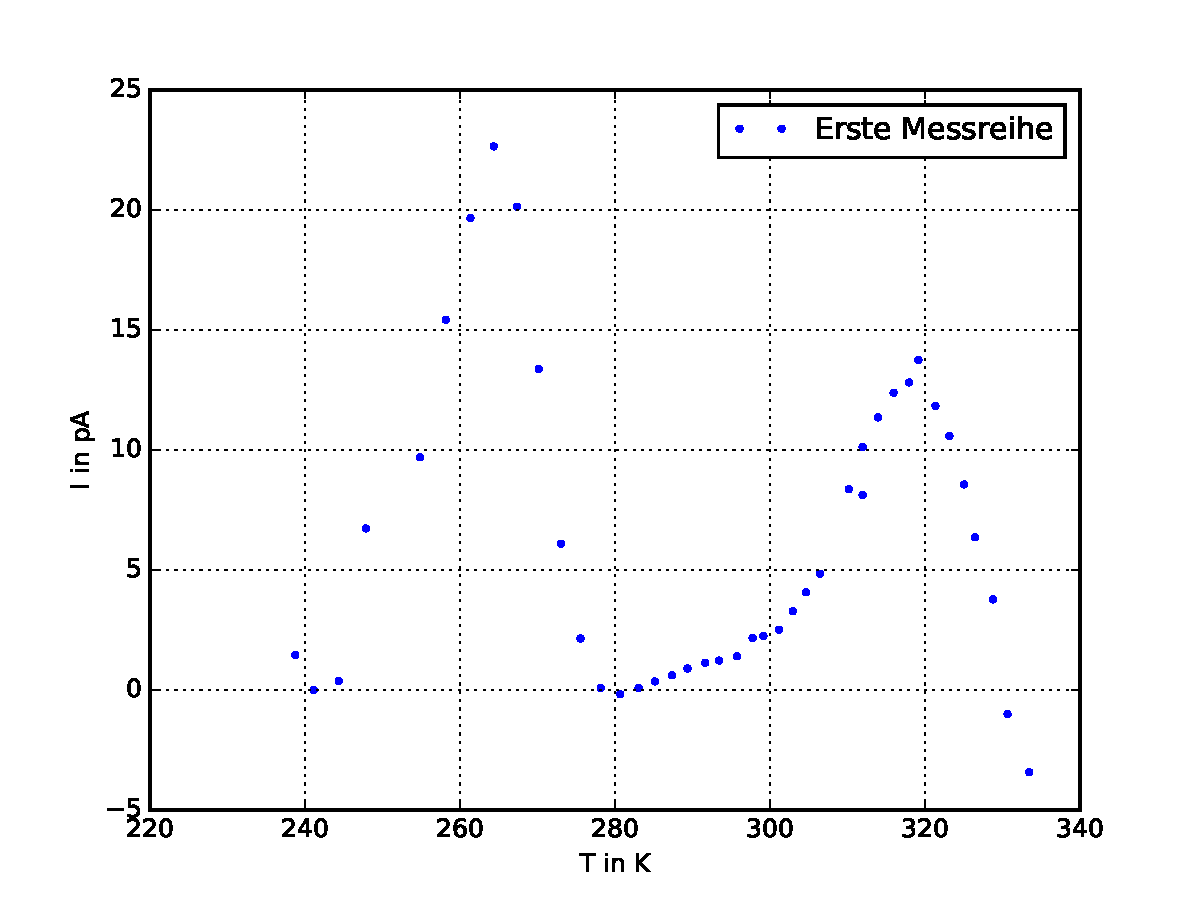
\includegraphics[height=6.2cm]{plots/ohneuntergrund.pdf}
   \caption{Messreihe 1}
   \label{fig:mess1o}
 \end{subfigure}
 \begin{subfigure}{0.48\textwidth}
   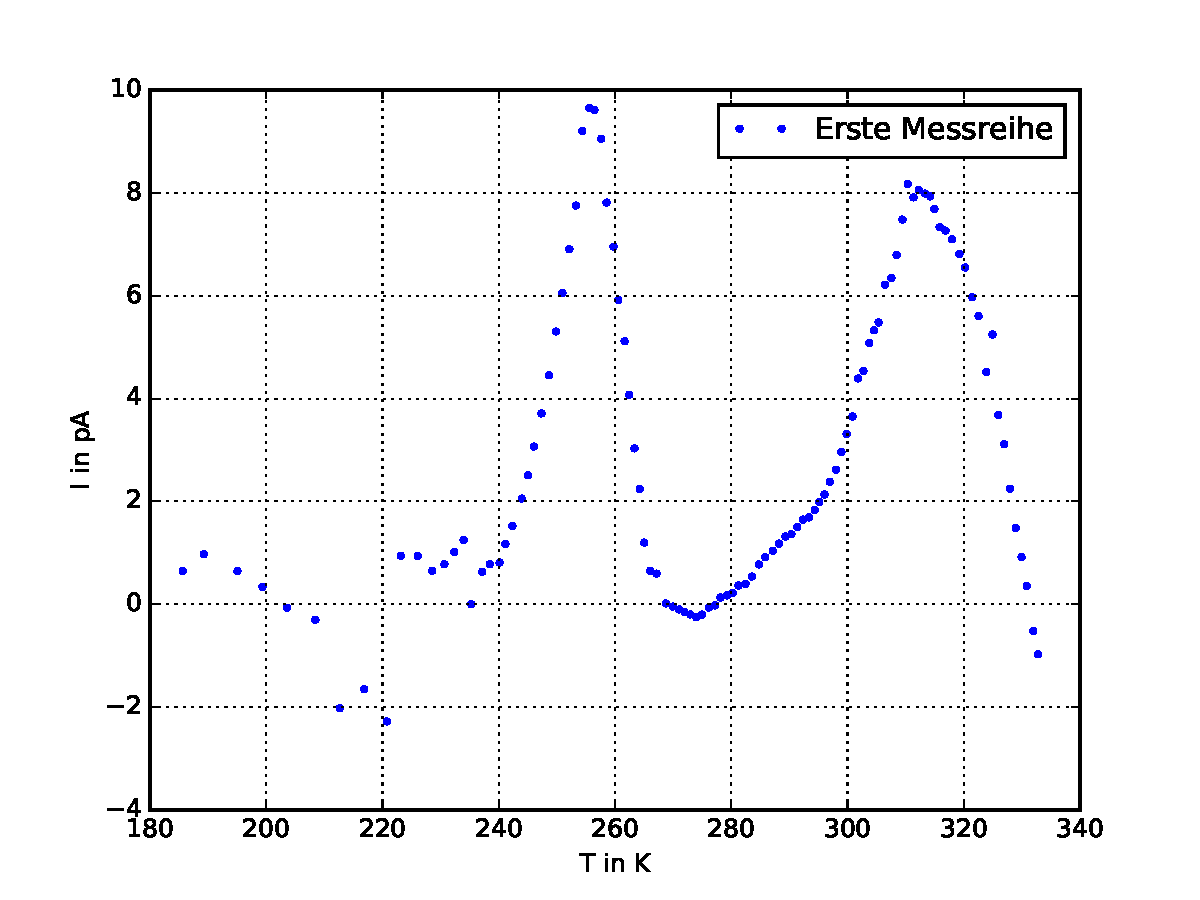
\includegraphics[height=6.2cm]{plots/ohneuntergrund2.pdf}
   \caption{Messreihe 2}
   \label{fig:mess2o}
 \end{subfigure}
 \caption{Darstellung der Messwerte für beide Heizraten nach Abzug des Untergrunds.}
 \label{fig:ohneunter}
\end{figure}

\subsection{Berechnung der Aktivierungsarbeit aus der Anlaufkurve}
Um die Aktivierungsarbeit der Dipole zu berechnen, wird eine Regression anhand der Messwerte für Temperatur und Strom mit einer Exponentialfunktion der Form
\begin{equation}
  y(T) = a\cdot e^{mT}
  \label{eqn:efit}
\end{equation}
erstellt.
% Mittlere heizspannung efit 3.2 0.13
\begin{figure}[H]
  \centering
  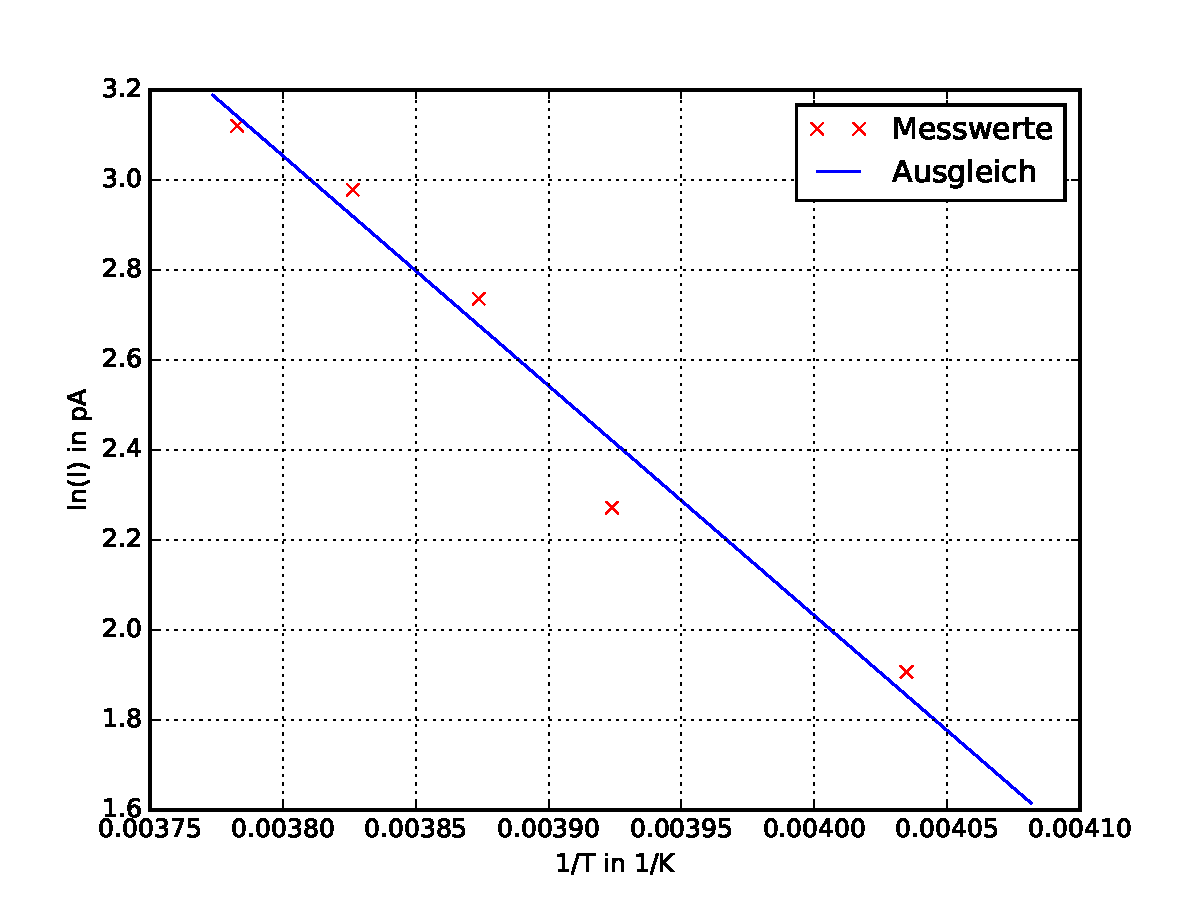
\includegraphics[width=0.8\textwidth]{plots/anlauf1.pdf}
  \caption{Anlaufkurve zu einer Heizrate von $H_1 =\SI{3.3 \pm 0.08}{\kelvin\per\minute}$.}
  \label{fig:anlauf1}
\end{figure}
\begin{figure}[H]
  \centering
  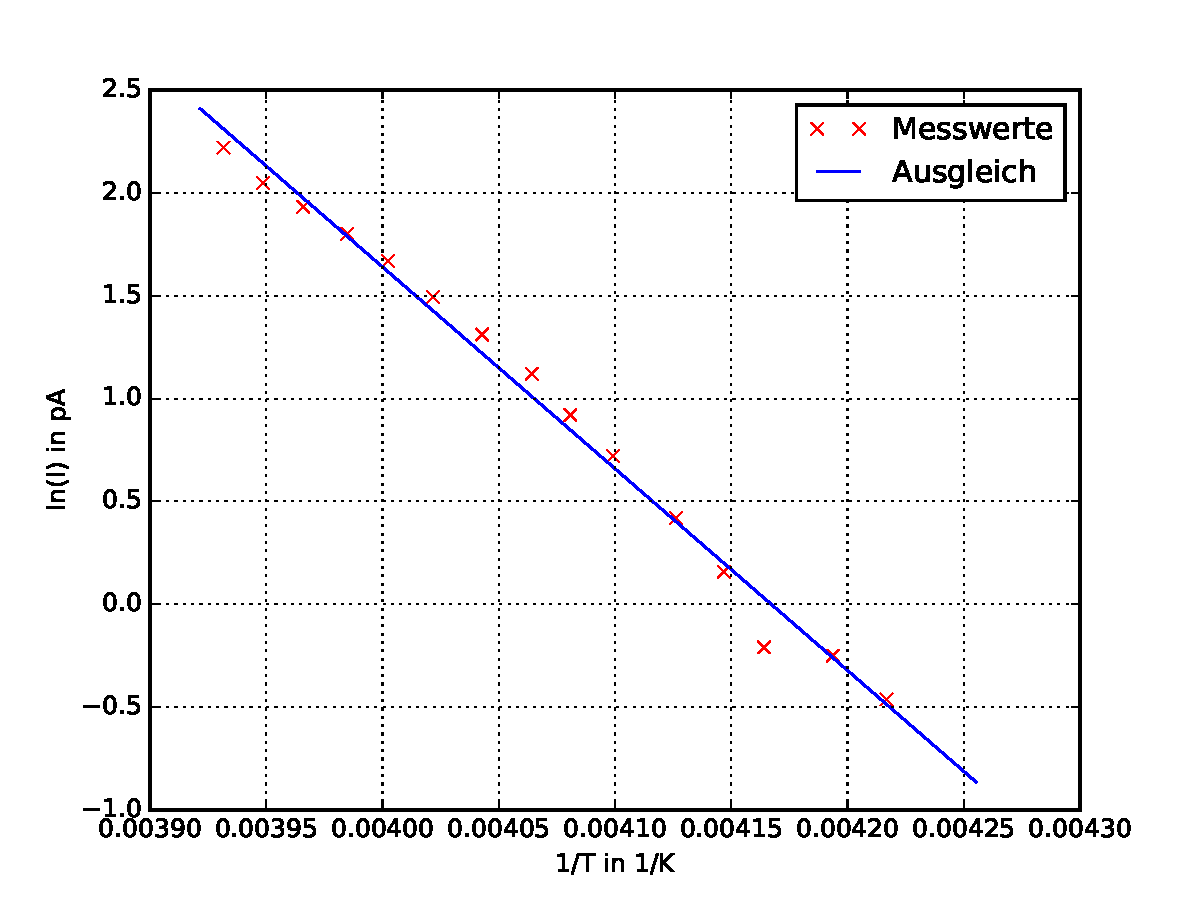
\includegraphics[width=0.8\textwidth]{plots/anlauf2.pdf}
  \caption{Anlaufkurve zu einer Heizrate von $H_2 =\SI{1.26 \pm 0.07 }{\kelvin\per\minute}$.}
  \label{fig:anlauf2}
\end{figure}
Die durch Ausgleichsrechnung erstellten Anlaufkurven sind in Abbildung \ref{fig:efit1} und \ref{fig:efit2} zu sehen.
Für die Kurve der zweiten Messung wurden die in Abbildung \ref{fig:efit2} gezeigten blauen Messwerte nicht berücksichtigt.
Aus den angehängten Messwerten wurden ausserdem mittlere Heizraten für beide Messungen bestimmt. Die aus den Werten der Anlaufkurve ermittelten Heizraten lauten:
\begin{center}
  $H_1 =(3.2 \pm 0.13)\frac{\symup{K}}{\text{min}}$, $H_2 = (1.26 \pm 0.064)\frac{\symup{K}}{\text{min}}$.
\end{center}
Aus der Ausgleichsrechnung ergeben sich die Parameter zu
\begin{center}
    $m_1 = 5680.23$, $ a_1= 24.98$, $m_2 = 5425.56$, $a_2 = 23.87$.
\end{center}
Aus dem Parameter $m_{(\symup{i})}$ werden dann nach
\begin{equation}
  W_{\symup{i}} = m_{\symup{i}}\cdot k_B
\end{equation}
die Austrittsarbeiten berechnet. Die berechneten Arbeiten lauten:
\begin{center}
  $W_1 = \SI{0.44}{\electronvolt}$ und $W_2 = \SI{0.84}{\electronvolt}$
\end{center}
\subsection{Berechnung der Aktivierungsenergie durch Integrieren}
Um die Aktivierungsarbeit präziser zu ermitteln, wird nun die ganze Strom-Temperatur-Kurve verwendet.
Im folgenden wird nun mit den vom Untergrund getrennten Daten erneut die Aktivierungsarbeit ermittelt.
Eine lineare Ausgleichsrechnung von $f(T) = \ln(\frac{\int_{T}^{T^*}i(T')\symup{d}T'}{i(T)})$ aufgetragen gegen $1/T$ liefert die Ausgleichsparameter:
\begin{center}
  $m_1 = 13248 \pm 1716$, $b_1 = -49.1\pm 6.6 $
  $m_2 = 12280 \pm 370$, $b_2=-46.9 \pm 1.5 $.
\end{center}
Die Ausgleichsrechnungen sind in den Abbildungen \ref{fig:log1} und \ref{fig:log2} für beide Heizraten dargestellt.
\begin{figure}[H]
  \begin{subfigure}{0.48\textwidth}
   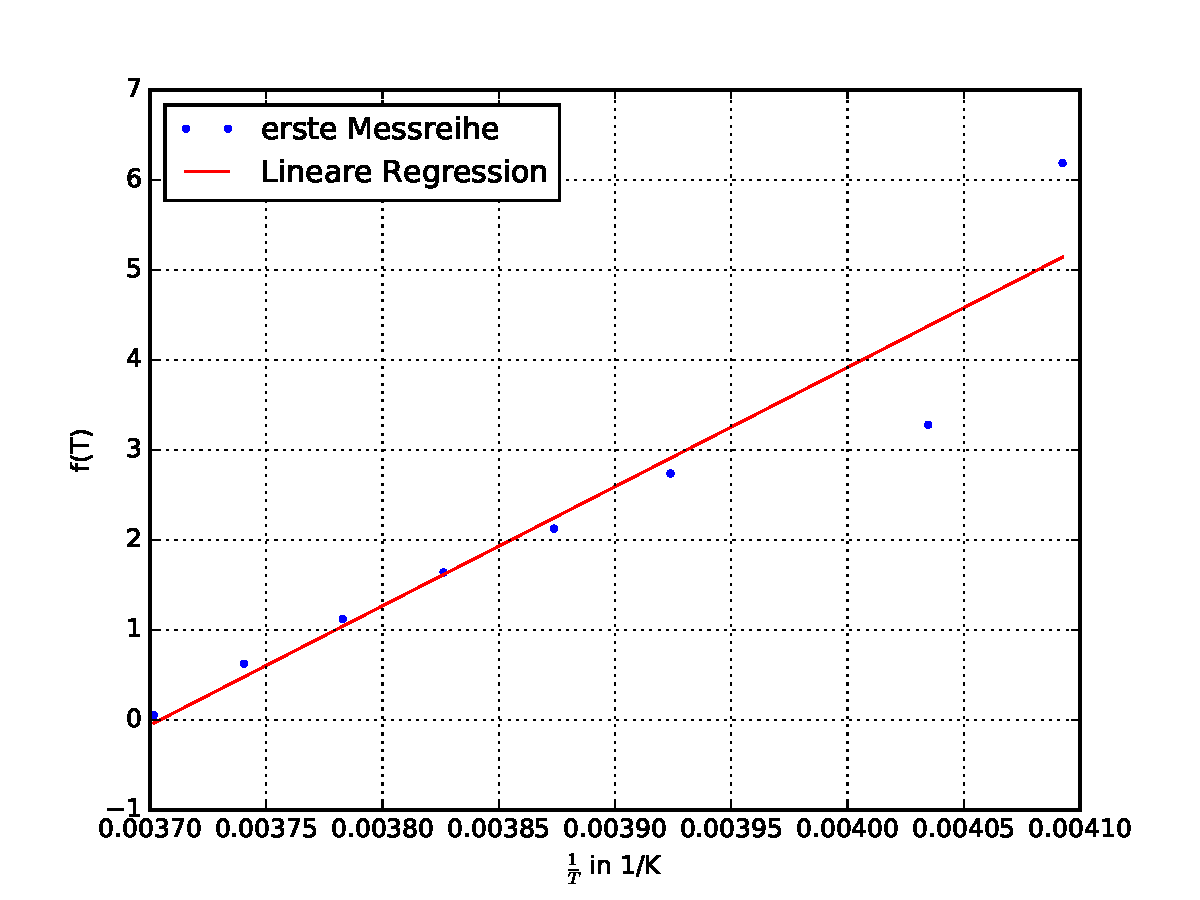
\includegraphics[height=6.2cm]{plots/integralplot1.pdf}
   \caption{Heizrate $H=3.2$.}
   \label{fig:log1}
 \end{subfigure}
 \begin{subfigure}{0.48\textwidth}
   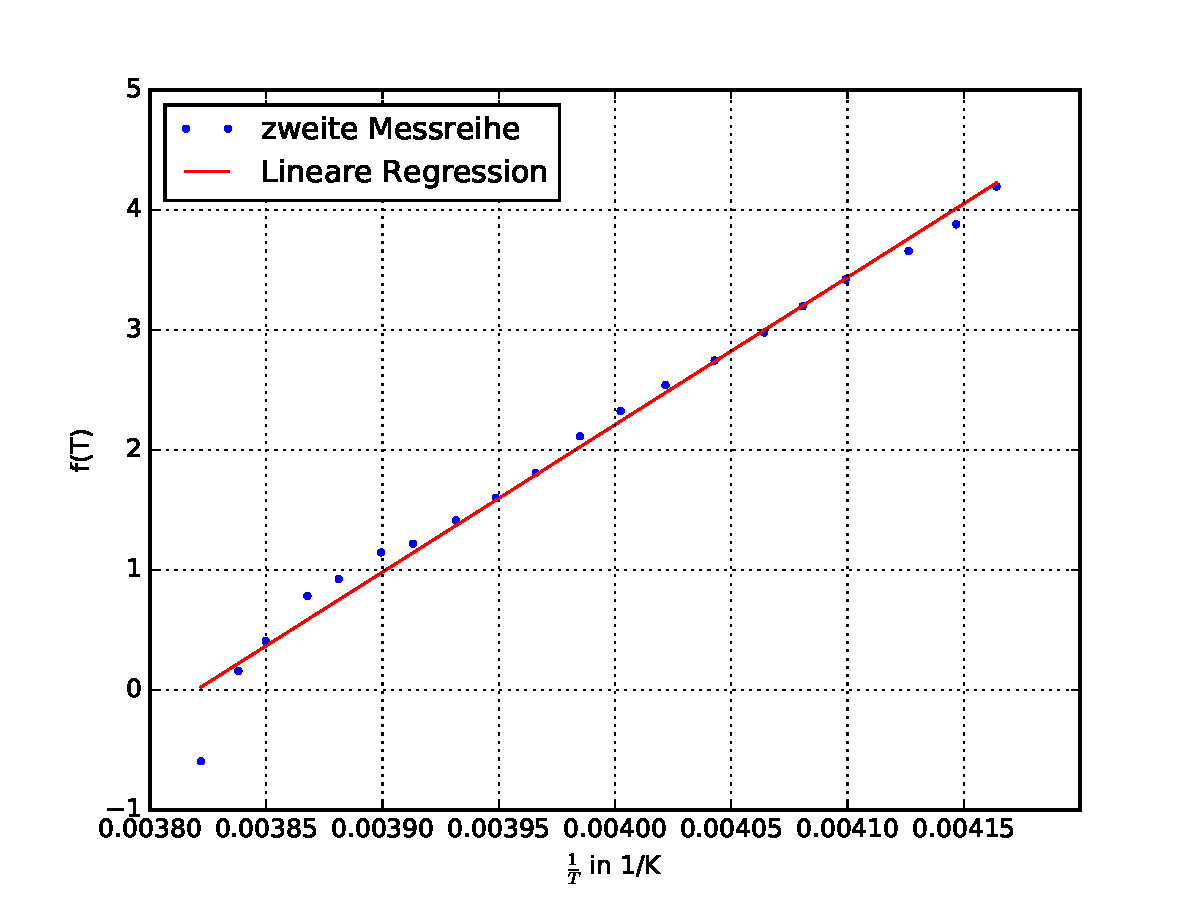
\includegraphics[height=6.2cm]{plots/integralplot2.pdf}
   \caption{Heizrate $H=1.26$.}
   \label{fig:log2}
 \end{subfigure}
 \caption{Lineare Ausgleichsrechnungen der Messwerte.}
\end{figure}
Da der Relaxationsprozess beim ersten Minimum in Abbildung \ref{fig:ohneunter} als abgeschlossen betrachtet wird, werden für die Integration nur die Messwerte im Bereich bis zu diesem Minimum verwendet.
Aus den Paramtern der Ausgleichsrechnung ergeben sich die Aktivierungsenergien zu
\begin{equation*}
  W_1^I = k_B m_1 = \SI{1.14}{\electronvolt},\,\,\, W_2^I = k_B m_2 = \SI{1.05}{\electronvolt}
\end{equation*}
% Für die zweite Messreihe ergibt sich entsprechend:
\subsection{Bestimmung der charakteristischen Relaxationszeit}
Aus Abbildung \ref{fig:mitunter} werden kene Temperaturen bestimmt, bei denen I maximal ist:
\begin{center}
  $T_{max,1} = \SI{-8.8}{\celsius}$ und $T_{max,2} = \SI{-16.7}{\celsius}$.
\end{center}
Mithilfe dieser Werte und den errechneten Aktivierungsenergien ergibt sich gemäß \eqref{eqn:tau3}:
\begin{center}
  $\tau_{max,1}   = \SI{4.27}{\second}$\\ $\tau_{max,2}   = \SI{5.28}{\second}$\\
  $\tau_{max,1}^I = \SI{4.22}{\second}$\\
  $\tau_{max,2}^I = \SI{5.69}{\second}$
\end{center}
Dieser Werte lassen sich wiederrum durch \eqref{eqn:relaxation} in $\tau_0$ überführen.
Dies liefert für die aus Anlaufkurve und Integration berechneten Aktivierungsenergien folgende Relaxationszeiten.
\begin{table}[H]
  \centering
  \caption{Aus Regression der Anlaufkurve und Integration ermittelte charakteristische Relaxationszeiten $\tau_0$.}
  \label{tab:relax}
  \begin{tabular}{c|c|c|c}
    Anlaufkurve&&Integration&\\
    \hline
    $\tau_{01}$ & $\tau_{02}$ & $\tau_{01}^I$ & $\tau_{02}^I$\\
    \hline
    $1.73\cdot 10^{-8}\si{\second}$ & $1.13\cdot 10^{-16}\si{\second}$ & $6.79\cdot 10^{-21}\si{\second}$ & $2.82\cdot 10^{-22}\si{\second}$\\
  \end{tabular}
\end{table}
